\documentclass{fefu_presentation}

\usepackage{graphicx}
\graphicspath{{images/}}

\usepackage{subcaption} % subfigure

\setgroup{М9999-99.99.99xxxx}
\setsupervisor{Петров Пётр Петрович}{учёная степень, учёное звание\\должность, место работы}
\setschoolreferencetitle{Института}
\setschooltitle{Институт}
\setschool{математики и компьютерных технологий}


\author{Иванов Иван Иванович}
\title{Название работы}
\date{\today}

%Enable notes page alongside the main page, that can be used similar to PowerPoint notes
%\enablenotes

\begin{document}
    
    \presentationtitlepage
    
    \note{Защищается студент группы М9999-99.99.99xxxx по теме название работы. Руководитель учёная степень, учёное звание Иванов Иван Иванович}
    
    \begin{frame}{Предметная область}
        \begin{block}{}
            При описании предметной области должны быть отражены
            \begin{itemize}
                \item Направление деятельности, которой посвящена работа, её актуальность, примеры задач
                \item Краткое описание части предметной области, непосредственно касающейся работы
                \item Описание проблем, актуальных для заказчика, а также примеры, статические факторы, подтверждающие наличие проблем
            \end{itemize}
        \end{block}
    \end{frame}

    \note{}
    
    \begin{frame}{Цель работы}
        \begin{block}{}
            Составить слайд с описанием цели и задач работы
        \end{block}
        \begin{block}{Задачи}
            \begin{itemize}
                \item Сформулировать цель
                \item Сформулировать не более 5 задач, обобщая мелкие при необходимости
                \item Оформить слайд
            \end{itemize}
        \end{block}
    \end{frame}

    \note{}
    
    \begin{frame}{Анализ существующих решений}
        \begin{block}{}
            \begin{itemize}
                \item Указать описание существующих решений
                \item Подробнее остановиться на наиболее существенных
                \item Привести сравнительную таблицу
            \end{itemize}
        \end{block}

        \begin{fefucomparisontable}
            \feature{convenient}{Удобно}
            \feature{free}{Бесплатно}
            \feature[3cm]{grade}{Можно получить оценку}

            \comparate{LaTeX}
            \convenient[$\pm$]
            \free
            \grade

            \comparate{PowerPoint}
            \grade

            \comparate{Не делать}
            \convenient
            \free

            \comparate{Лист бумаги}
        \end{fefucomparisontable}
    \end{frame}

    \note{}

    \begin{frame}{Функциональные требования}
        \begin{block}{}
            Привести описание функциональных требований к разрабатываемому решению
        \end{block}
    \end{frame}

    \note{}

    \begin{frame}{Математическая модель}
        \begin{block}{}
            \begin{itemize}
                \item Привести краткое описание математической модели, выделив результаты, полученные в рамках работы
                \item При оформлении математических формул необходимо описать на слайде все переменные, используемые в них
                \item Для неоригинальных формул привести источники
            \end{itemize}
        \end{block}
        \begin{block}{Эквивалентность массы и энергии\footnote{Эйнштейн 1905}}
            \begin{equation}
                E=mc^2
            \end{equation}

            \centering
            \begin{tabular}{ll}
                $E$ --- энергия & $m$ --- масса\\
                $c$ --- скорость звука&\\
            \end{tabular}
        \end{block}
    \end{frame}

    \note{}

    \begin{frame}{Проектные решения}
        \begin{block}{}
            Перечислить и кратко обосновать принятые решения в отношении
            \begin{itemize}
                \item методов, алгоритмов, структуры кода
                \item программных и аппаратных средств реализации
            \end{itemize}
        \end{block}
        \begin{block}{}
            Продемонстрировать на слайдах и пояснить
            \begin{itemize}
                \item структуру данных, диаграмму классов, архитектуру системы
                \item проект интерфейса в виде 3--7 снимков экрана
            \end{itemize}
        \end{block}
    \end{frame}

    \note{}
    
    \begin{frame}{Примеры оформления слайдов презентации}
        \begin{figure}[h]
            \centering
            \begin{subfigure}[t]{0.49\textwidth}
                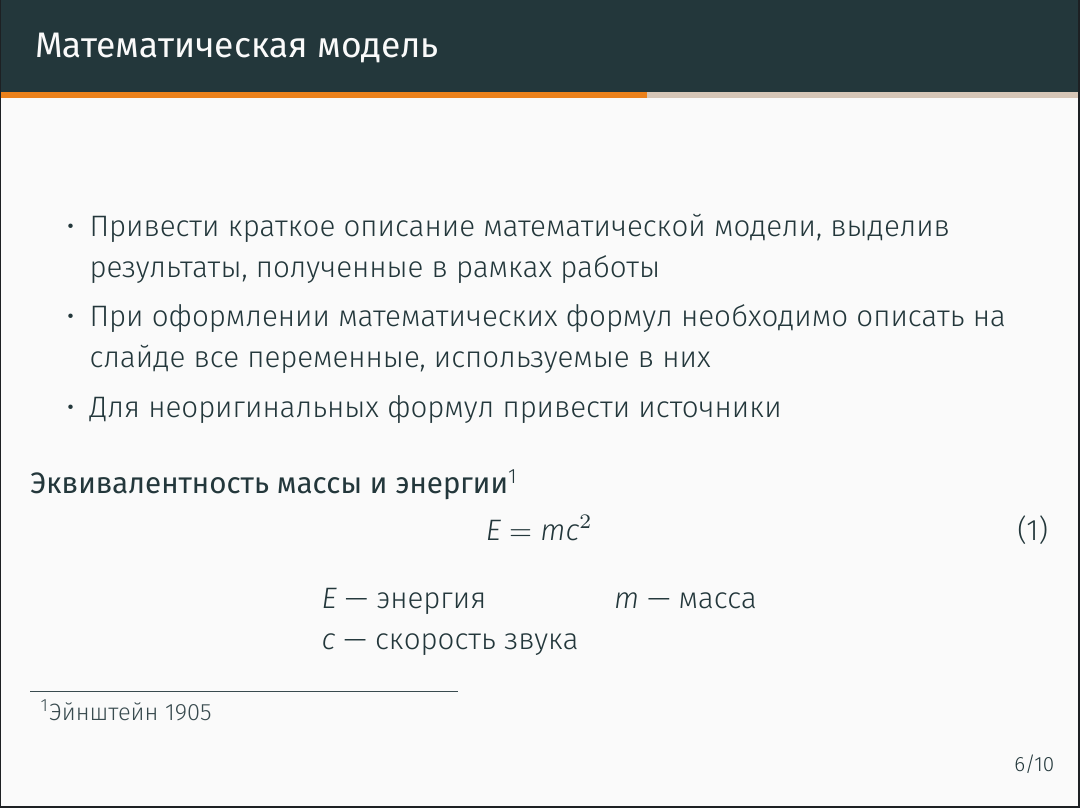
\includegraphics[width=\textwidth]{slide1.png}
                \caption{Математическая модель}
            \end{subfigure}
            \begin{subfigure}[t]{0.49\textwidth}
                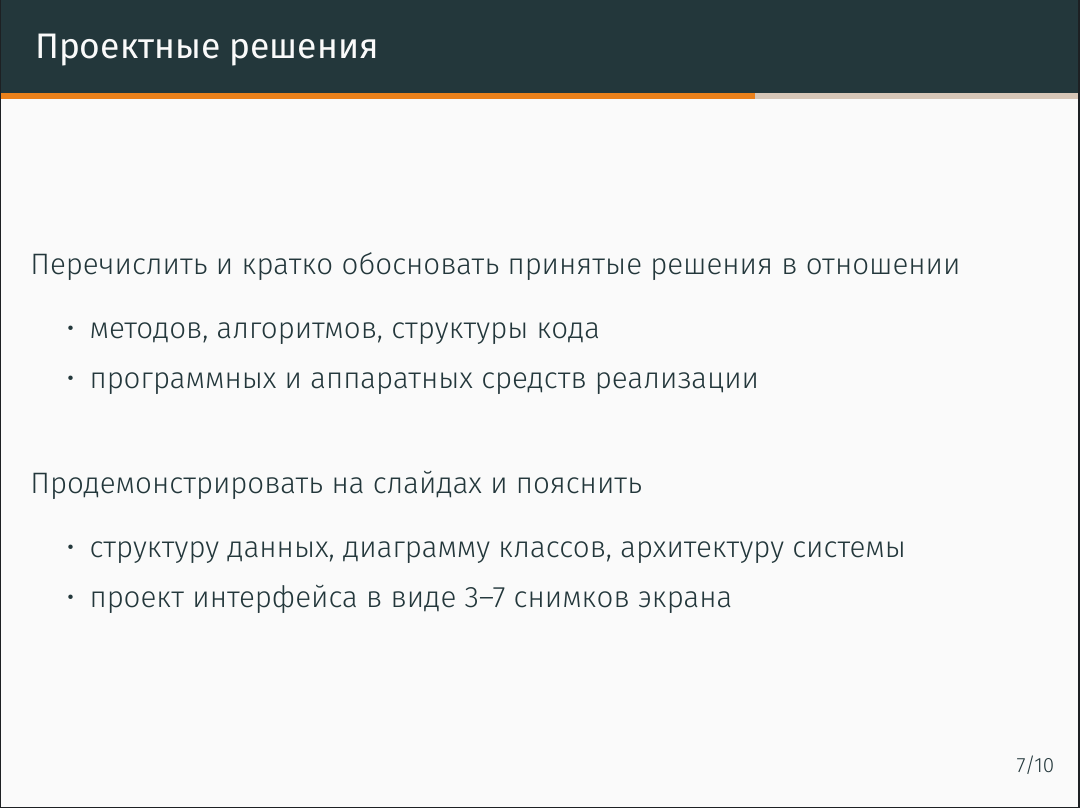
\includegraphics[width=\textwidth]{slide2.png}
                \caption{Проектные решения}
            \end{subfigure}
        \end{figure}
    \end{frame}

    \begin{frame}{Реализация и тестирование}
        \begin{block}{}
            \begin{itemize}
                \item Привести физические характеристики программного продукта на слайде
                \item Описать методику и результаты тестирования
                \item В случае наличия вычислительного эксперимента, привести соответствующие графики, диаграммы и выводы
            \end{itemize}
        \end{block}
    \end{frame}

    \note{Физические характеристики разработанной системы (внесённых доработок) приведены на слайде}

    \begin{frame}{Заключение}
        \begin{block}{}
            \begin{itemize}
                \item Перечислить основные результаты, достигнутые во время работы
                \item Описать перспективы дальнейшего использования и совершенствования продукта
                \item Выделить наиболее важные результаты работы
            \end{itemize}
        \end{block}
    \end{frame}

    \note{СПАСИБО ЗА ВНИМАНИЕ}
    
\end{document}
